\chapter{\label{sec:experimentation-and-evaluation}Experimentation and Evaluation}

% - trust explorer example
% - 9 fully functional modules
% - demonstrate the viability of run-time changes and alternative algorithmic approaches
% - open questions:
%   - how do we evaluate this?
%   - how do we show that it works as intended?
%   - we successfully bypassed the Android security model with protection against dynamic code injection using Webview
%   - pure technical (module loading times, memory usage impact, event-driven impact, event processing workload analysis, peak performance estimation)
%   - Github/NodeJS/Debian replacement workload analysis ("github is the largest code host in the world, with 20 million users and more than 57 million repositories"

This chapter will propose an experiment and evaluate the framework described in Section~\ref{sec:design}. The evaluation will be performed based on the result gathered from the experiment.

\section{Experiment}

The experiment consists out of conducting a use-case study, by creating a fully functioning example that demonstrates the composition and construction of an application with interchangeable trust models. This application will consist out of 6 components:

\begin{itemize}
	\item Test application GUI (view layer)
	\item Test application (logic layer)
	\item Trust algorithm 1 (logic layer)
	\item Trust algorithm 2 (logic layer)
	\item Execution engine (infrastructure layer)
	\item Transport engine (infrastructure layer)
\end{itemize}

Figure~\ref{fig:experiment} shows an overview of the example application. The domain of trust was chosen since this is a very interesting use-case that has not been explored yet in other works. It allows users of a system to define their own notion of the concept of trust and apply this to their system without requiring extensive knowledge about each application they are using. For this experiment, this work makes use of two different trust algorithms: Netflow and PimRank. These two algorithms act as an exampl for this experiment.

\begin{figure}[h]
	\centering
	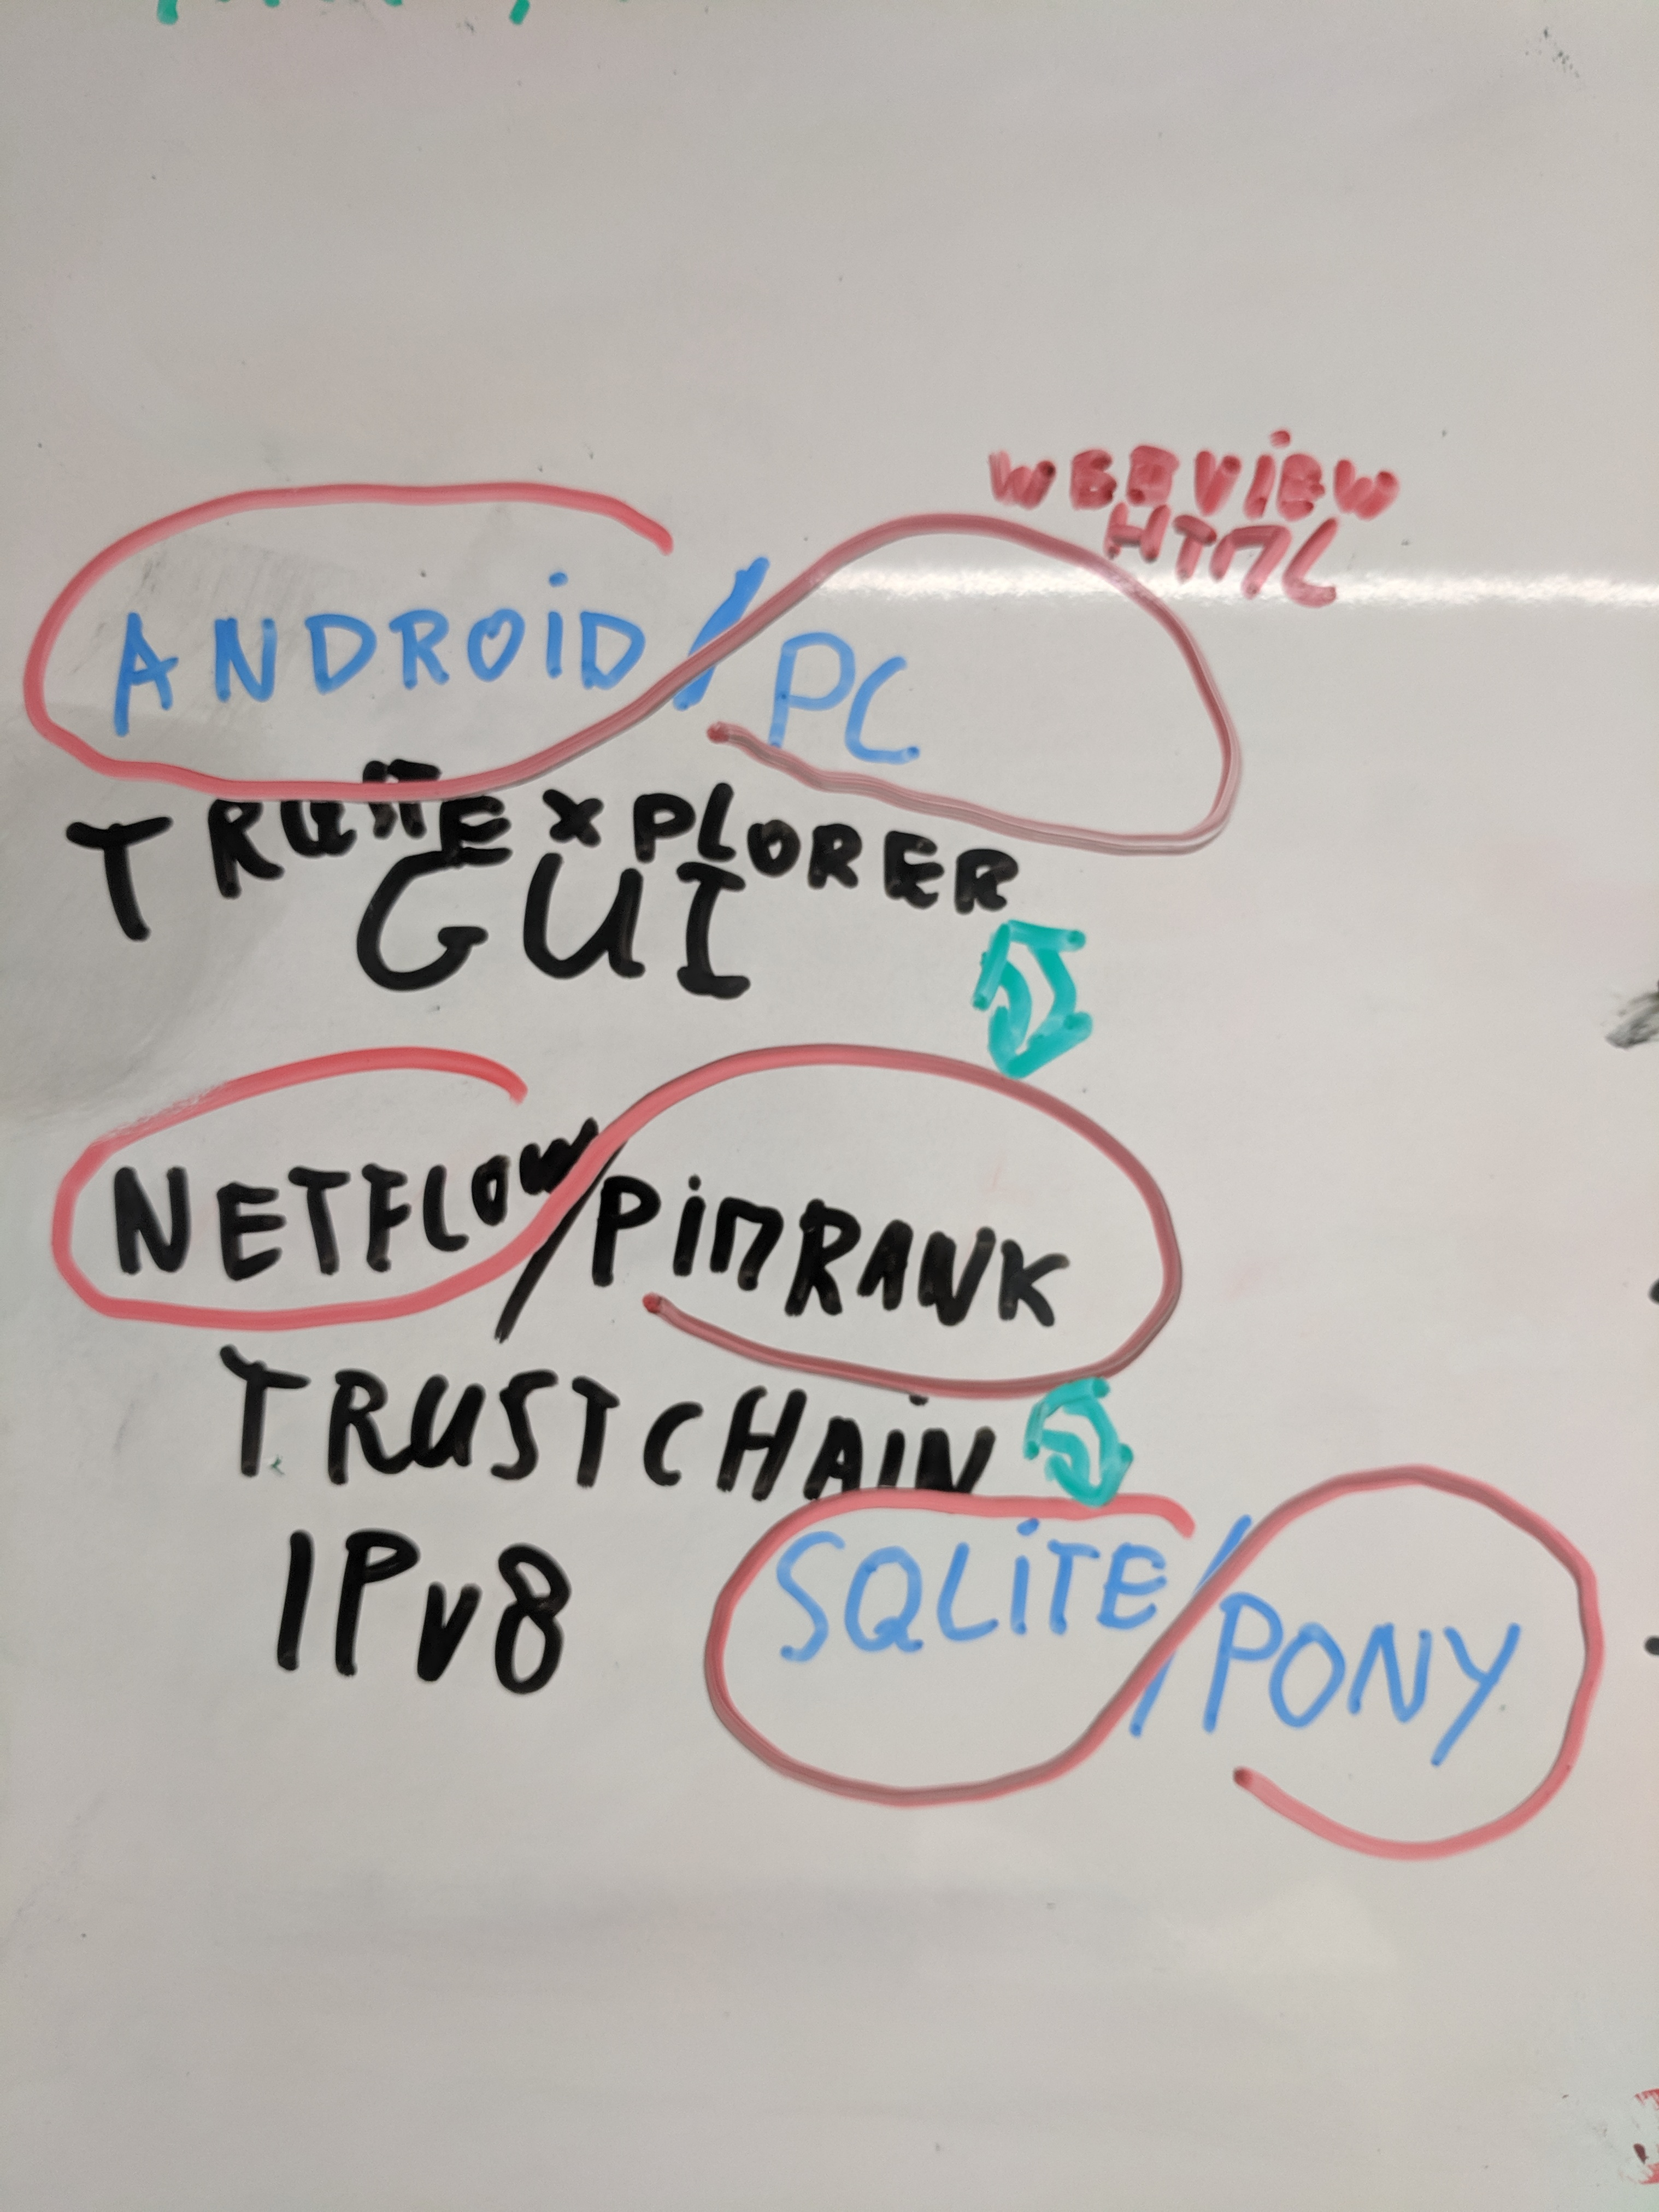
\includegraphics[width=0.5\textwidth]{images/experiment.jpg}
	\caption{\label{fig:experiment}}
\end{figure}

\section{Mobile App}

To test the robustness and the flexibility of the framework, an experiment was performed to try to create a proof-of-concept prototype of an Android application that could run the same stack of code to extend the ecosystem to mobile platforms. Since the two major mobile platforms (Android, iOS) only run applications custom made for these platforms, different methods had to be explored. Because iOS has a very restricted development environment and strict security policies, this route was not further explored.

The Android platforms allows app developers to run Java, Kotlin (Java based), and C. The desired framework language (Python) does not natively run on this platform. Converting the project code and dependencies is not a simple or maintainable method. This approach, however, also would not work. To improve security, the Android platform makes use of app scanning to verify that the executables haven't been tampered with. This security method severly hinders the working of the framework, since more functionality is added by distribution of application through its peer-to-peer network. These new code inclusions would trigger warnings in the Android security system and would block the app.

To circumvent this, a un-official method was used to package all the necessary code, dependencies, and executables as a single file and execute this as a C service on the Android platform. To accomplish this, a project called Python-for-Android was used. Python-for-Android is a build script that compiles the desired Python system version and Python dependencies for the ARM platform and creates a directory structure that can be used to run on Android. In Figure~\ref{fig:android-architecture} and overview of the Android app structure can be seen.

\begin{figure}[h!]
	\centering
	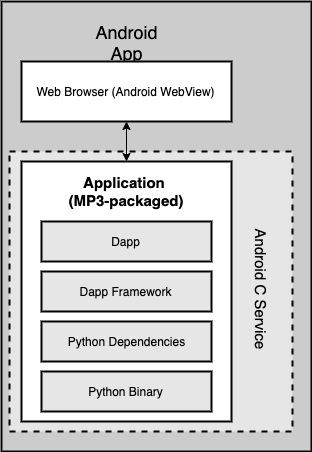
\includegraphics[width=0.5\textwidth]{images/android-app.png}
	\caption{\label{fig:android-architecture}}
\end{figure}

Since the Android app is needed to interact with the C service in the background, a part of the app had to be written in either Java or Kotlin. To keep this amount of code to a minimum, a decision was made to create all GUIs in web technologies, so the view layer can be shared between mobile and desktop platforms. This decision made it possibly to include a web browser as the only component written for the mobile platform. This web browser can then interact with the web server and REST API running on the C service.

To package the executable code in a way that would not trigger the Android security system, the code had to be bundled in a single file, disguised as a MP3. This format does not get checked by the Android security system  and therefore can be used for the purpose of this work. Underneath the extenstion, the code is packaged as a GZIP Tar-archive. Upon running the Android application, this MP3 file is unpacked in the application space of the app and the C service is started with the right configuration to run the code.

In Figure~\ref{fig:android-app} a screenshot can be seen of the framework running with a test dApp on the Android platform. Development was stopped after reaching the proof-of-concept stage as it is not the main goal of this work and the development cycle is very tedious and slow. Each time a change or addition is made to the Framework the entire app structure has to be rebuild. This process can take up to 20 minutes. 

\begin{figure}[h!]
	\centering
	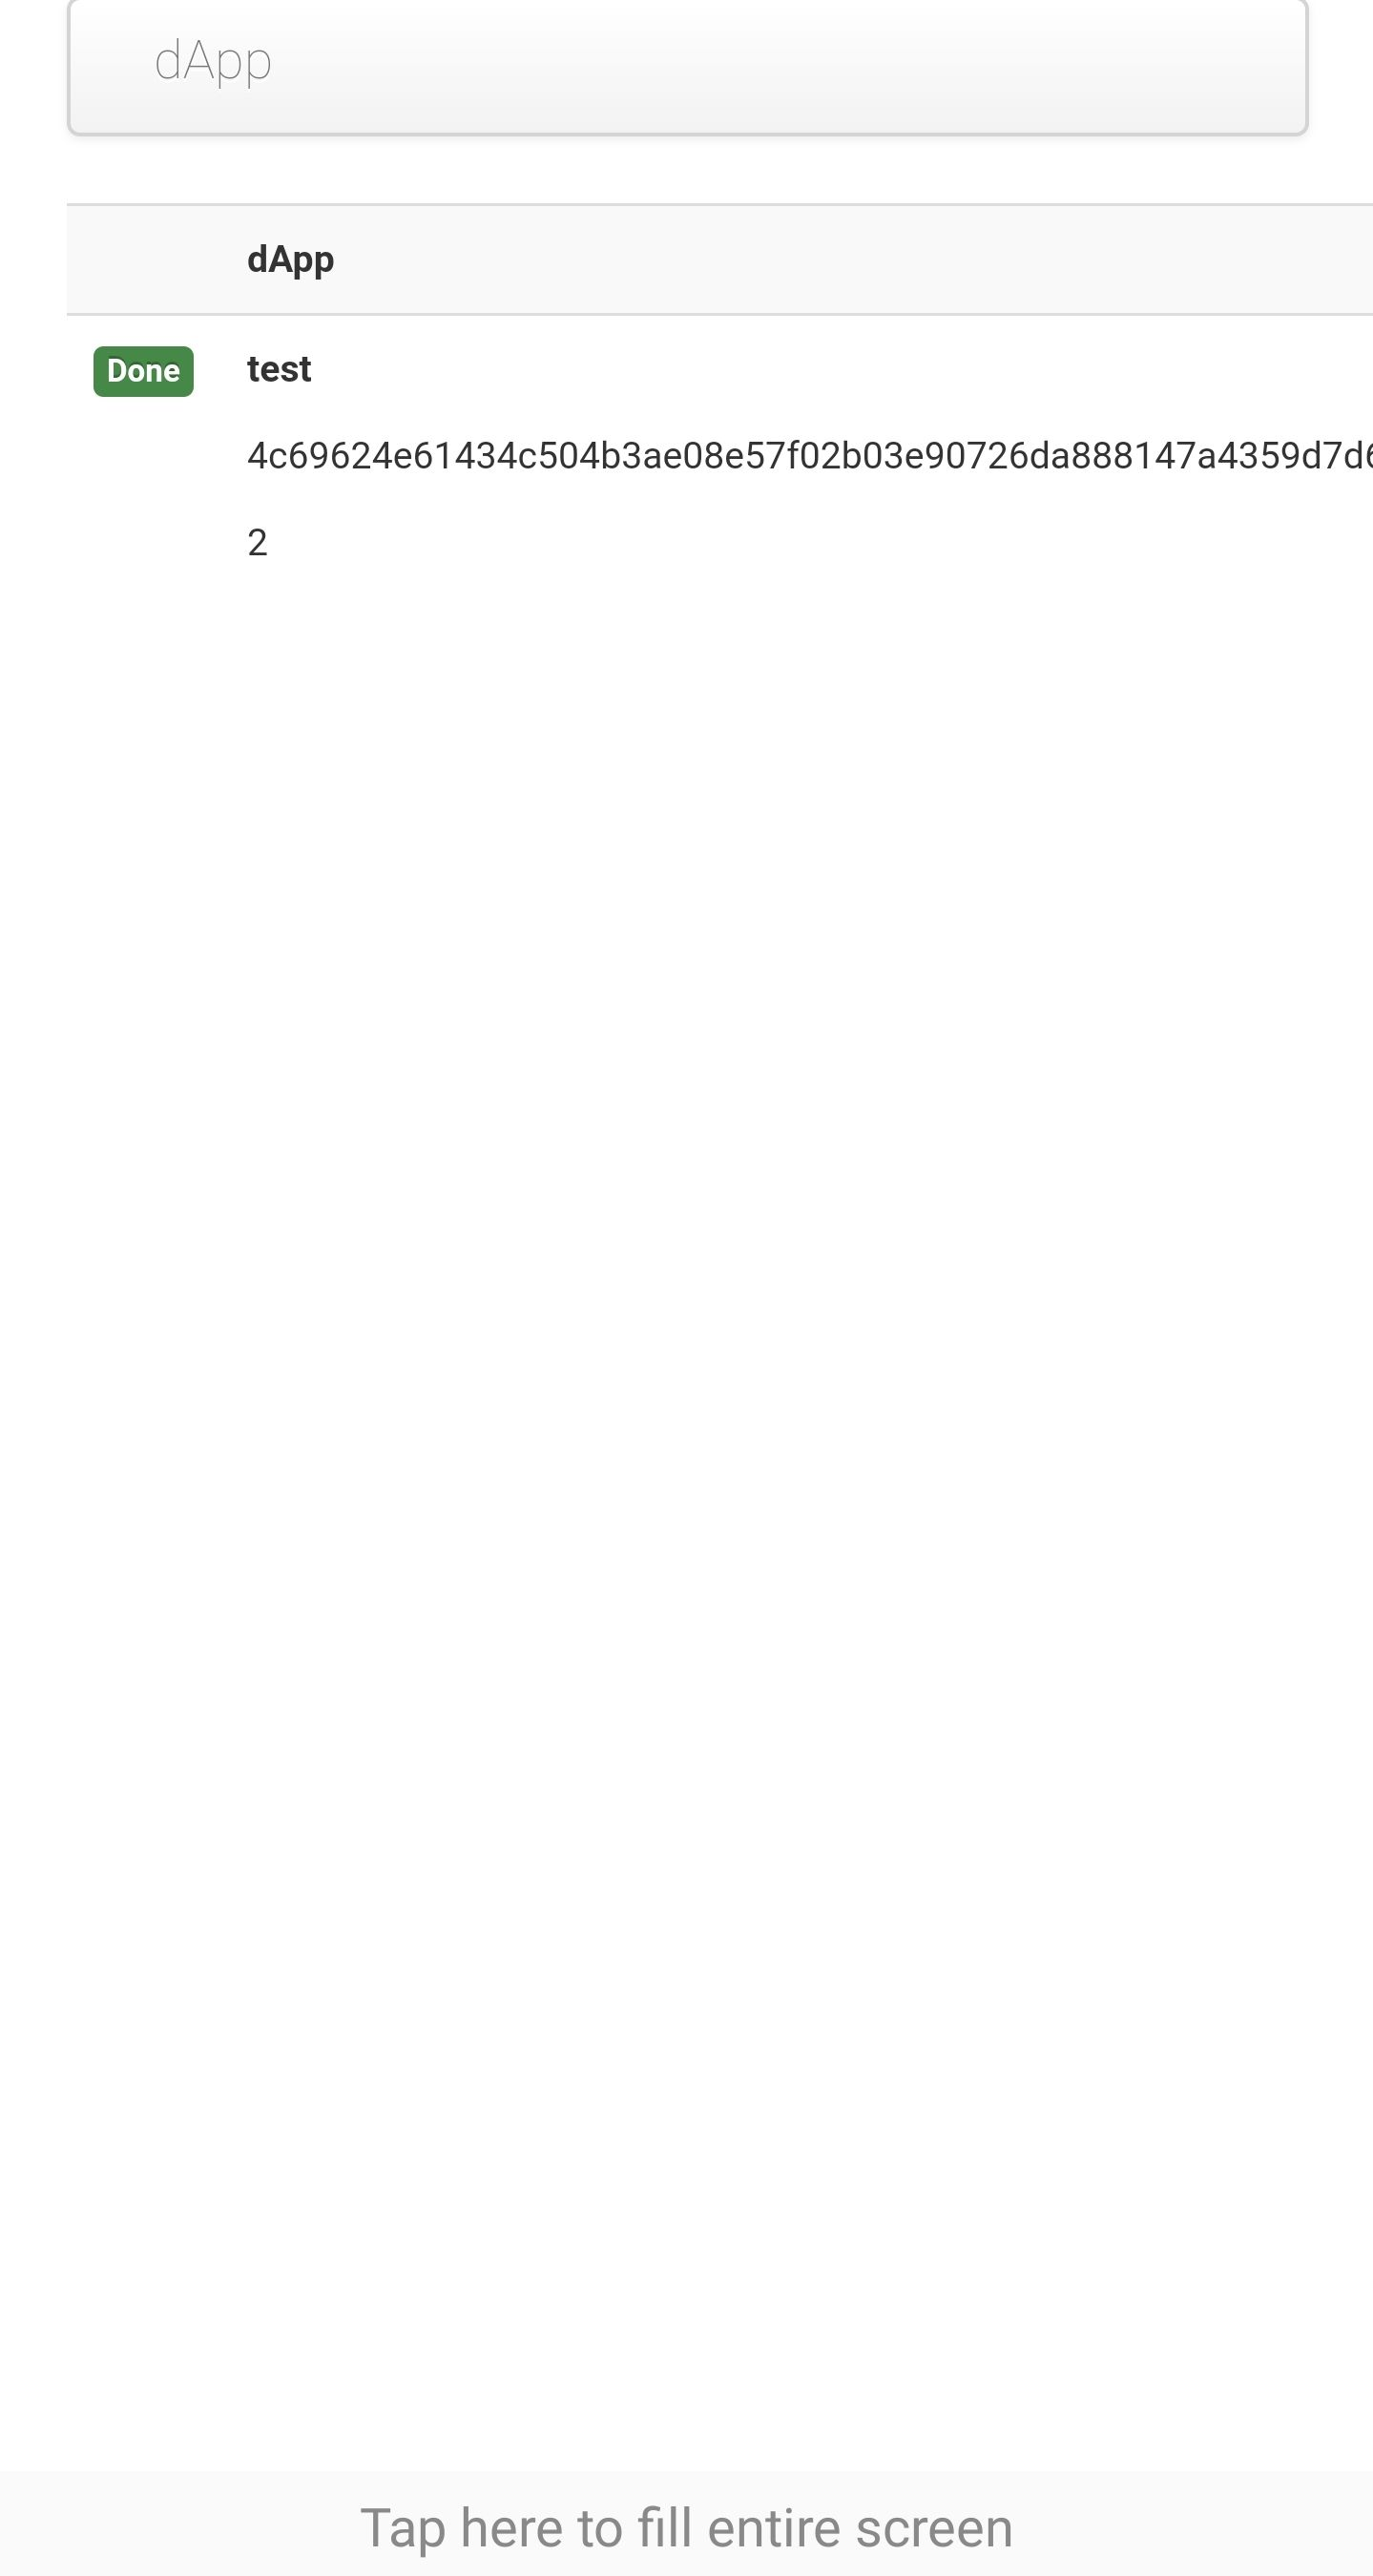
\includegraphics[width=0.5\textwidth]{images/android-app-screenshot.jpg}
	\caption{\label{fig:android-app}}
\end{figure}



%\section{Tribler}
%
%% Project focuses on project called Tribler. Community driven. Big code base.
%
%Tribler is an open-source community driven decentralized BitTorrent client being developed and researched at the Delft university of Technology. Its main feature is that is allows anonymous peer-to-peer communication by default. It is built on the underlaying network library IPv8, also being worked on by the same group.
%
%Besides handling the tasks of a standard BitTorrent client, Tribler also makes it possible to:
%
%\begin{itemize}
%	\item \textbf{Search for content: } allowing the program to operate independently of external content search providers that could be blocked and maked it immune to limiting external actions such as legal constraints. Which is happening more frequently nowadays.
%	\item \textbf{Torrent anonymously: } routing torrent traffic through anonymized tunnels that operate using the same principle as the TOR stack. Providing pseudo-anonymity for the two end and other observing parties.
%	\item \textbf{Accumulate trust: } all torrenting metadata is stored in a way that is not linked to an physical identity or an IP address. This data is then translated into a trust score by calculating the ratio between the amount of traffic communicated across the network. A positive seed ratio (the ratio between uploading content and downloading content) indicated a positive trust value.
%	\item \textbf{Trade trust: } With this trust system it is possible to prioritize or refuse services for particular users. To increase the incentive for having a large seeder network and therefore a high trust value, Tribler allows users with a large amount of uploaded content to exchange this gathered trust for currency on the built-in marketplace inside the Tribler application.
%\end{itemize}
%
%This trust value, expressed as reputation inside the Tribler application, can be described as an up- and download currency in a reputation-based peer-to-peer network. When a peer uploads more than it downloads, the reputation of that peer increases, and the peer can download more effectively.
%
%\section{IPv8}
%
%IPv8 is the underlying network framework of the Tribler application. It is responsible for providing \textbf{authenticated} and \textbf{encrypted} communication between different peers (computer nodes) in the system. The framework abstracts the notion of physical addresses (IP addresses) in favour of public keys. This removes the need for application that use this framework to keep track of where different peers in the system are and how to move data between them. IPv8 simplifies the design of distributed overlay systems. 
%
%Some other important aspects of the framework are its focus on:
%\begin{itemize}
%	\item \textbf{Privacy:} where it is possible to choose if messages should be identifiable to all peers in the network or only to the peers absolutely needed for the network connection (doesn't include the receiver). 
%	\item \textbf{No infrastructure dependency:} allowing the network to function on its own run by the peers using the system. This is a very important aspect of the framework as it allows the framework to support itself, without needing external financing for server capacity.
%	\item \textbf{NAT traversal:} making it possible to operate the network without static servers needed for overcoming the NAT issues that most peer-to-peer networks face.
%	\item \textbf{Trust:} one of the most important aspects of peer-to-peer systems, as it is needed to mitigate free-riding issues in the network. In IPv8 trust is gained by recording a patterns of previous actions and storing these on a blockchain structure called TrustChain.
%\end{itemize}

%The last main aspect of the framework is \textbf{extensibility}. IPv8 makes use of a concept called overlays. Where a virtual network is created in the system related to one specific application domain or topic where different peers can subscribe to. This is a very powerful mechanism to allow extendability and modularization of an specific application.